% Options for packages loaded elsewhere
\PassOptionsToPackage{unicode}{hyperref}
\PassOptionsToPackage{hyphens}{url}
\PassOptionsToPackage{dvipsnames,svgnames,x11names}{xcolor}
%
\documentclass[
  12pt,
]{article}
\usepackage{amsmath,amssymb}
\usepackage{lmodern}
\usepackage{iftex}
\ifPDFTeX
  \usepackage[T1]{fontenc}
  \usepackage[utf8]{inputenc}
  \usepackage{textcomp} % provide euro and other symbols
\else % if luatex or xetex
  \usepackage{unicode-math}
  \defaultfontfeatures{Scale=MatchLowercase}
  \defaultfontfeatures[\rmfamily]{Ligatures=TeX,Scale=1}
\fi
% Use upquote if available, for straight quotes in verbatim environments
\IfFileExists{upquote.sty}{\usepackage{upquote}}{}
\IfFileExists{microtype.sty}{% use microtype if available
  \usepackage[]{microtype}
  \UseMicrotypeSet[protrusion]{basicmath} % disable protrusion for tt fonts
}{}
\makeatletter
\@ifundefined{KOMAClassName}{% if non-KOMA class
  \IfFileExists{parskip.sty}{%
    \usepackage{parskip}
  }{% else
    \setlength{\parindent}{0pt}
    \setlength{\parskip}{6pt plus 2pt minus 1pt}}
}{% if KOMA class
  \KOMAoptions{parskip=half}}
\makeatother
\usepackage{xcolor}
\usepackage[left=3cm,right=2cm,top=2cm,bottom=2cm]{geometry}
\usepackage{graphicx}
\makeatletter
\def\maxwidth{\ifdim\Gin@nat@width>\linewidth\linewidth\else\Gin@nat@width\fi}
\def\maxheight{\ifdim\Gin@nat@height>\textheight\textheight\else\Gin@nat@height\fi}
\makeatother
% Scale images if necessary, so that they will not overflow the page
% margins by default, and it is still possible to overwrite the defaults
% using explicit options in \includegraphics[width, height, ...]{}
\setkeys{Gin}{width=\maxwidth,height=\maxheight,keepaspectratio}
% Set default figure placement to htbp
\makeatletter
\def\fps@figure{htbp}
\makeatother
\setlength{\emergencystretch}{3em} % prevent overfull lines
\providecommand{\tightlist}{%
  \setlength{\itemsep}{0pt}\setlength{\parskip}{0pt}}
\setcounter{secnumdepth}{5}
\usepackage{mathtools}
\usepackage{amsmath}
\numberwithin{equation}{section}
\numberwithin{table}{section}
\numberwithin{figure}{section}
\usepackage{float}
\usepackage{gensymb}
\usepackage{setspace}\singlespacing
\usepackage{titlesec}
\titlespacing*{\section}{0pt}{3cm}{1cm}
\usepackage[nottoc]{tocbibind}
\setcounter{secnumdepth}{2}
\setcounter{tocdepth}{2}
\widowpenalties 3 10000 10000 150
\displaywidowpenalties 3 10000 10000 150
\clubpenalties 3 10000 10000 150
\interfootnotelinepenalty 5000
\raggedbottom
\usepackage{enumitem}
\setlist{itemsep=3pt,topsep=5pt,parsep=0pt,partopsep=0pt}
\usepackage{hyperref}
\hypersetup{bookmarksnumbered=true}
\usepackage{bookmark}
\newcommand{\sectionbreak}{\clearpage\phantomsection}
\let\Begin\begin
\let\End\end
\newcommand{\Newrow}{\\}
\AtBeginDocument{\pdfbookmark[section]{Cover Page}{front}}
\usepackage{booktabs}
\usepackage{longtable}
\usepackage{array}
\usepackage{multirow}
\usepackage{wrapfig}
\usepackage{float}
\usepackage{colortbl}
\usepackage{pdflscape}
\usepackage{tabu}
\usepackage{threeparttable}
\usepackage{threeparttablex}
\usepackage[normalem]{ulem}
\usepackage{makecell}
\usepackage{xcolor}
\ifLuaTeX
  \usepackage{selnolig}  % disable illegal ligatures
\fi
\usepackage[]{natbib}
\bibliographystyle{agsm}
\IfFileExists{bookmark.sty}{\usepackage{bookmark}}{\usepackage{hyperref}}
\IfFileExists{xurl.sty}{\usepackage{xurl}}{} % add URL line breaks if available
\urlstyle{same} % disable monospaced font for URLs
\hypersetup{
  pdftitle={Asessing China's Climate Responsibility},
  pdfauthor={Johann-Friedrich Salzmann},
  colorlinks=true,
  linkcolor={MidnightBlue},
  filecolor={Maroon},
  citecolor={MidnightBlue},
  urlcolor={MidnightBlue},
  pdfcreator={LaTeX via pandoc}}

\title{Asessing China's Climate Responsibility\\
\strut \\
\strut \\
\strut \\}
\usepackage{etoolbox}
\makeatletter
\providecommand{\subtitle}[1]{% add subtitle to \maketitle
  \apptocmd{\@title}{\par {\large #1 \par}}{}{}
}
\makeatother
\subtitle{\textbf{Final Paper}\\
\strut \\
\strut \\
GRAD-E1402\\
Data Perspectives on GHG Emissions\\
Hertie School of Governance\\
\strut \\}
\author{submitted by\\
Meier, Constantin\\
Metz, Fabian\\
Mohn, Anna\\
Salzmann, Johann-Friedrich\\
\strut \\}
\date{12 December 2022}

\begin{document}
\maketitle

\renewcommand{\harvardand}{\&}
\renewcommand{\harvardurl}{\textbf{URL:} \url}
\setcitestyle{authoryear,round,aysep={},notesep={: }}

\nocite{R-rmarkdown,R-tidyverse,R-eurostat,R-WDI,R-plotly,R-imputeTS,R-kableExtra}

\thispagestyle{empty}
\pagenumbering{gobble}

\newpage
\pdfbookmark[section]{List of Abbreviations}{decl}
\section*{List of Abbreviations}
\thispagestyle{empty}
\pagenumbering{arabic} 
\onehalfspacing

\begin{table}[!ht]
    \centering
    \begin{tabular}{|l|l|}
    \hline
        AFOLU &  Agriculture, Forestry, Land Use  \\ \hline
        CAT &  Climate Action Tracker  \\ \hline
        CBRD &  Common but differentiated responsibilities and respective capabilities  \\ \hline
        COP &  Conference of the Parties  \\ \hline
        EDGAR &  Emissions Database for Global Atmospheric Research  \\ \hline
        GDP &  Gross domestic product  \\ \hline
        GHG &  Greenhouse gas  \\ \hline
        GNI &  Gross national income  \\ \hline
        GW &  Gigawatt  \\ \hline
        NDC &  Nationally determined contributions  \\ \hline
        REDD+ &  Reducing Emissions from Deforestation and Forest Degradation  \\ \hline
        UNFCCC & United Nations Framework Convention on Climate Change \\ \hline
    \end{tabular}
\end{table}

\singlespacing
\newpage
\pdfbookmark[section]{\contentsname}{toc}
\tableofcontents
\thispagestyle{empty}
\onehalfspacing

\hypertarget{introduction}{%
\section{Introduction}\label{introduction}}

The development that the People's Republic of China has taken in recent
decades is nothing short of remarkable. While the country, under the
dictatorial leadership of Mao Zedong, was plagued by poverty and famine
during the first three decades after its founding in 1949, Deng
Xiaoping's policy of reform and opening started the country's economic
boom in the late 1970s. Millions of Chinese have made the leap out of
poverty since, and the country, which at the beginning of the 21st
century was still considered the ``workbench of the world'', has now
developed into an economic and technological superpower that is readying
itself to overturn the global supremacy of the U.S..

During the same period, China's emissions have risen rapidly. In 2004,
the country surpassed the U.S. as the world's largest greenhouse gas
emitter and is likely to retain that title for some time. In 2019, more
than 25\% of all global greenhouse gas emissions came from China, more
than the U.S. and (at the time still) EU-28 combined (see Figure 1). As
a consequence of this development, China's emissions profile changed
dramatically: While the agricultural sector still accounted for a large
share of emissions in the early 1970s, its contribution has been only
marginal in recent years. Figure 2 shows the large-scale
industrialization of the country starting in the mid-1990s and the
corresponding increase in emissions from the energy sector. More
recently, transport sector emissions have picked up speed, likely
reflecting the wealthy share of China's citizens spending more money on
individual (fossil-fuel based) modes of transport.

China's energy mix is still largely dominated by coal. In 2020, more
than 60\% of the country's total energy supply stemmed from this fossil
fuel. Renewables on the other hand only contributed 6.2\% to total
energy supply (excluding biofuel and waste). Looking at just the
electricity production, the numbers are a bit different: Here the
renewable sources' share was approx. 28\% \citep{IEA2022}. However,
China remains the country with the world's largest coal fleet and also
the highest planned coal capacity additions. In 2021, the country
started building 33 GW of additional coal-based power generation and
consumed about five times as much coal as India, and nearly six times as
much as the U.S. \citep{Green2022}.

Chinese carbon emissions growth was predominantly driven by its rapid
economic development, which in turn caused the energy sector to grow
too. Since the year 2000, China's GDP per capita has more than
quadrupled, while carbon emissions have more than tripled in the same
period (see Figure 3). However, the growth of emissions has slowed in
recent years, as energy intensity of GDP had started decreasing after
the year 2005 and also carbon intensity of energy peaked in 2010 and has
been slowly decreasing since. While for the first two decades of the
21st century carbon emissions growth rates were closely resembling the
growth rates of GDP per capita, since 2010 the two numbers have
decoupled. China's immense expansion of renewable energy sources over
the last years is likely an underlying driver of this trend, however, as
we have seen, Chinese annual emissions remain very high at 14.2 GtCO2e
in 2019.

The question arises, how China plans to curb its emissions. At the
United Nations General Assembly in 2020, Chinese President Xi Jinping
announced the goal of Chinese carbon neutrality before 2060
\citep{Jinping2020}. This was the first time China officially committed
to a long-term emissions reductions goal \citep{CAT2022}. One year
later, in November 2021, ahead of COP26, China submitted its updated NDC
to the UNFCCC. Accordingly, the country plans to peak its carbon
emissions before 2030, decrease the carbon intensity of GDP by over 65\%
(relative to 2005), have around 25\% of non-fossil fuels in primary
energy consumption by 2030, increase the forest stock volume by six
billion cubic meters until 2030 and have 1,200 GW of wind and solar
power capacity installed by the same year \citep{China2022}. Although
some of these objectives are vague to some degree, and the emissions
reduction target is only a relative goal, the ambitions China has set
for itself are a marked improvement over the targets set out in the
previous 2016 NDC. Additionally, it is important to note that these
goals are unconditional and hence not relying on external climate
finance. China has adopted numerous policies to support its
international targets, such as the ``Working Guidance for Carbon Dioxide
Peaking and Carbon Neutrality'' and the ``Action Plan for Carbon Dioxide
Peaking Before 2030''. The former spells out a set of principles and
sectoral goals to achieve carbon dioxide peaking and carbon neutrality,
among them the need to exercise nationwide planning and the
prioritization of conversing energy (Department of Resource Conservation
and Environmental Protection, 2021a). The latter defines key tasks for
driving the low-carbon energy transition or saving energy, carbon
emission mitigation and efficiency improvement \citep{DRCEP2021b}. With
its ``14th Five-Year Plan on Renewable Energy'', the country aims to
further accelerate its renewable energy expansion. By 2025, 33\% of
electricity ought to be supplied by renewable sources (18\% non-hydro),
which could decrease annual carbon emissions by 2.6 gigatons
\citep{Zhou2022}.

Nonetheless, China's goals and policies are widely viewed as inadequate
by various parties. The CAT for example projects that China is likely to
comfortably overachieve its NDC targets without substantially increasing
its current mitigation efforts. Hence, their overall rating of the
country's goals and policies is ``insufficient''. If all countries were
to pursue the same level of ambition as China, global warming would
reach approx. 3°C. Therefore, China's current goals and policies leave
significant room for further target-raising ambition. The CAT
additionally concludes that China's contributions are also not
sufficient to do its ``fair-share'' in fighting climate change and
limiting global warming under the Paris Agreement \citep{CAT2022}.

China itself assesses its responsibility for climate change mitigation
measures very differently though. In its 2021 NDC update, China assigns
responsibility for global warming to developed countries. It were their
emissions that had caused the dramatic increase of GHGs in the
atmosphere. China, on the other hand, was a developing country, thereby
having the right to develop \citep{China2022}.

This line of argument is as old as the UNFCCC itself. In 1992, at the
first COP in Rio de Janeiro, where the parties agreed on the UNFCCC,
they classified countries into two groups of ``Annex-I'' and ``non-Annex
I'' countries, consisting of mostly developed and (at the time)
developing countries respectively. At the same time the principle of
common but differentiated responsibilities and respective capabilities
(CBRD) was introduced. According to this principle, the industrialized
nations would need to bear the main responsibility when it comes to
emission reductions, while the ``non-Annex I'' countries would initially
have no obligations to avoid emissions. This principle was also
enshrined in the 1997 Kyoto Protocol. The 2015 Paris Agreement
reaffirmed the CBRD principle, but, for the first time, brought all
signatory countries together to undertake ambitious efforts to tackle
climate change and adapt to its impacts \citep{UNFCCC2015}. However, it
has caused long-standing debates, whether China should continue to be
classified as a developing country, given its economic and emissions
growth since the UNFCCC was adopted, or whether it has a greater
responsibility in addressing climate change.

With these developments in mind and following up on China's claim to be
a developing country, we set out in this paper to discuss equity
considerations for China, focusing on two research questions. First, we
will investigate whether China, from an emissions perspective, can still
be characterized as a developing nation. For this we compare China's
Kaya identity with other developing and developed nations. Furthermore,
we consider China's sectoral emissions trends and contrast them with
those of (other) developing and developed nations, controlling for
differences in population size and GDP. Secondly, we investigate China's
claim of developed countries' being the driver of climate change, by
calculating different measures of (historic) responsibility and assess
the level of responsibility China bears in combatting climate change. We
discuss these findings with regards to a projection of China's
cumulative emissions.

The remainder of this paper is structured as follows: In section 2 we
provide an overview of our data and main assumptions, before analyzing
China's self-characterization as a developing country in section 3.
Section 4 compares different equity metrics for China and other big
emitters and discusses China's role in addressing climate change against
different scenarios of future Chinese cumulative emissions. In section 5
we discuss our findings in light of other available assessments of
China's role and conclude.

\begin{figure}
\centering
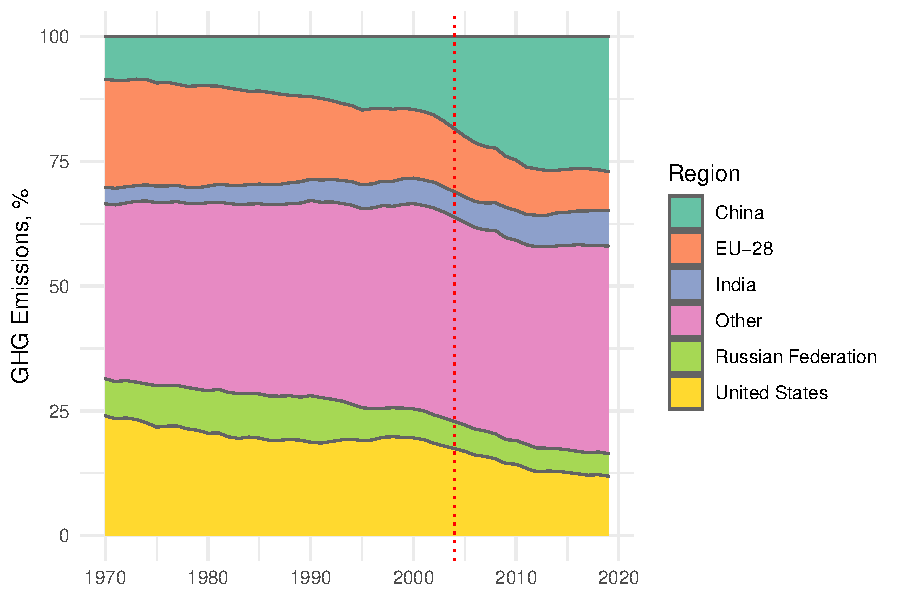
\includegraphics{Paper_files/figure-latex/unnamed-chunk-1-1.pdf}
\caption{Figure 1}
\end{figure}

\begin{figure}
\centering
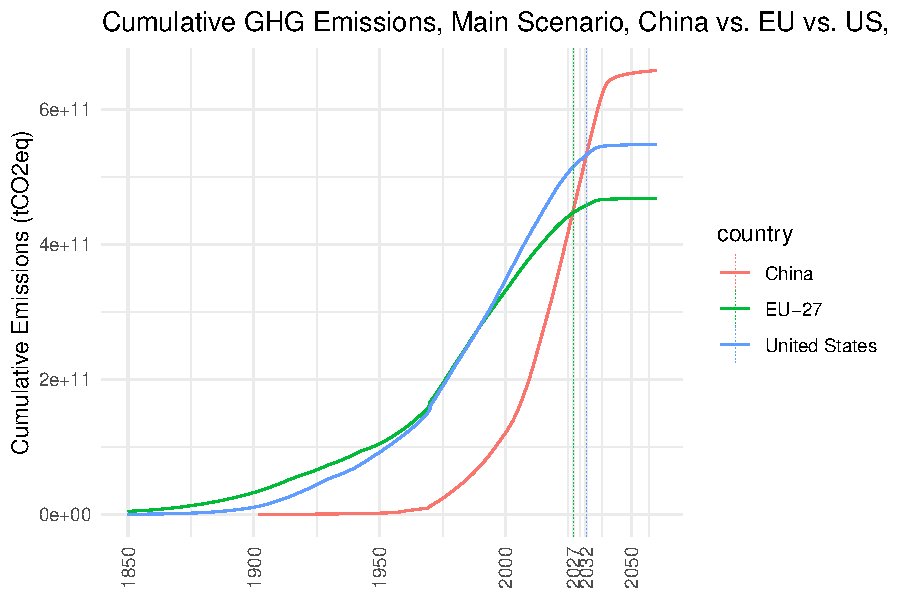
\includegraphics{Paper_files/figure-latex/unnamed-chunk-2-1.pdf}
\caption{Figure 2}
\end{figure}

\begin{figure}
\centering
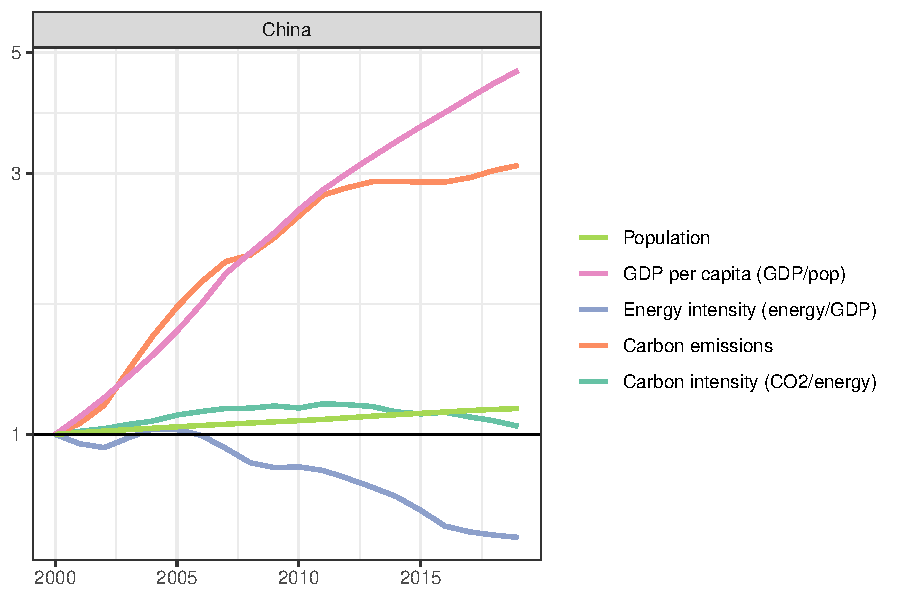
\includegraphics{Paper_files/figure-latex/unnamed-chunk-3-1.pdf}
\caption{Figure 3}
\end{figure}

\hypertarget{data-assumptions}{%
\section{Data \& Assumptions}\label{data-assumptions}}

Our project is data-driven in nature and relies heavily on the
availability of various metrics on both greenhouse gas emissions and
measures of (economic) development. Furthermore, there are key
assumptions connected to our analysis that impact our findings. This
section provides an overview of the data-sets we use, and makes our
underlying assumptions about the data explicit.

\hypertarget{used-data}{%
\subsection{Used Data}\label{used-data}}

In terms of data on GHG emissions we make use of the EDGAR database as
the core of our analysis. It contains yearly emissions data on the major
greenhouse gases by country and sector and makes them commensurable
based on global warming potentials on a 100-year scale. The database and
its development are a joint project of the European Commission Joint
Research Center and the Netherlands Environmental Assessment Agency
\citep{EC2022}.

We supplemented this data set with data on LULUCF emissions from the
national GHG inventory database and add them to the total GHG emissions.
The data itself was sourced from annual GHG inventories for Annex I
countries and gathered from recent communications, biennial update
reports, REDD+ submissions and NDCs for Non-annex I countries
\citep{Giacomo2022}.

For consumption-based emissions of selected countries since 1990 we make
use of an updated dataset from Peters et. al \citep[updated
from][]{Peters2011}. Additionally, we rely on world bank data for GDP,
GNI and population \citep{WorldBank2022d}. We further hand code
variables for countries, specifically their membership to the EU 27 \&
28 respectively, as well as their income classification according to the
2019-word-bank-classification for gross national income per capita
\citep{WorldBank2018}. Lastly two datasets were made available to us a)
an inventory of CO2 emissions since 1750 and b) IEA data for energy
consumption.

\hypertarget{general-assumptions}{%
\subsection{General Assumptions}\label{general-assumptions}}

Regarding our main assumptions we limit our analysis to years until 2019
as we believe that the pandemic heavily distorted prior trends and hit
countries and their economies to varying extents, making any meaningful
interpretation and comparison difficult. Our main assumption here is
that the trends and developments up to 2019 are more meaningful
indicators for developments in the years and decades to come, compared
to the pandemic years.

To make information accessible and to allow for comparisons across gases
we choose to provide all information on multiple GHGs based on 100-year
global warming potentials, as provided in our core database EDGAR.

\hypertarget{analysis}{%
\section{Analysis}\label{analysis}}

TO BE DONE: Intro statement.

\hypertarget{chinas-self-characterization-as-a-developing-country}{%
\subsection{China's Self-Characterization as a Developing
Country}\label{chinas-self-characterization-as-a-developing-country}}

In the following, China's self-characterization as a developing country
will be critically reviewed from an emissions perspective. For this, a
definition of developed and developing countries will be developed. This
is followed by a comparison of China's emissions development with the
emissions development of other developed and developing nations by using
a Kaya decomposition. As the distribution of emissions by sector is
another way to distinguish between developing and developed countries,
China's sectoral emissions are also compared to other countries. With
this, we strive to find an answer to our first research question.

\hypertarget{categorization-of-developed-and-developing-countries}{%
\subsubsection{Categorization of Developed and Developing
Countries}\label{categorization-of-developed-and-developing-countries}}

To distinguish between developed and developing countries, different
indicators can be considered for instance GDP per capita, the gross
national income GNI per capita or the human development index (HDI).
Furthermore, other indicators such as the level of education or
democracy can be taken into account when determining whether a country
is developed, developing or underdeveloped \citep{Kinnunen2019}.

Our main data set, the EDGAR dataset, already provides a classification
of countries in two groups -- developed and developing -- which we will
use as a starting point. According to this, China is categorized as a
developing country. However, we realized that a more granular
categorization of countries might be helpful to answer our first
research question. Especially since any type of self-categorization
might be biased as countries stand to gain from underestimating their
development in order to receive more aid and have less responsibilities
in the UNFCCC process.

Thus, we decided to use a second country classification scheme for
comparison. Although a financial indicator might not completely
summarize a country's level of development, we decided to use the GNI
cut-offs as our main indicator of development. This is mainly because
research finds that the GNI correlates with a number of accepted
indicators of development outcomes \citep{Fantom2016}. Furthermore, the
income classification is the standard classification in discussions on
development. The World Bank, but also other international organizations
and aid agencies, use this for analytical and operational purposes. The
GNI is calculated in the following way:

TO BE DONE FOrmula

Thus, going forward we will also use the World Bank's Classification of
Countries by income, which assigns countries into four different groups:
high income, upper-middle income, lower-middle income, low income.
Income is measured using the GNI per capita of the previous year in U.S.
dollars using a three-year average exchange rate. The classification is
updated each year. For our analysis, we are using the threshold valid as
of July 2019, as our emissions analysis considers this year as the last
year. The thresholds are as follows:

\begin{table}[!ht]
    \centering
    \begin{tabular}{|l|l|}
    \hline
        \textbf{Group  } & \textbf{Thresholds July 2019 in USD  } \\ \hline
        Low income   & $< 1,026$ \\ \hline
        Lower-middle income   & $1,026 - 3,955$ \\ \hline
        Upper-middle income  & $3,966 - 12,375$ \\ \hline
        High income  & $> 12,375$ \\ \hline
    \end{tabular}
\end{table}

According to the World Bank's classification, China is classified as an
upper-middle income country since 2010 \citep{WorldBank2022d}.

To make use of the more granular look at country groups in relation to
our research question, we assume low- and lower-middle income countries
to be more likely resembling developing nations and middle-upper- and
high-income countries to be more likely resembling developed nations.

\hypertarget{comparison-of-kaya-identities}{%
\subsubsection{Comparison of Kaya
Identities}\label{comparison-of-kaya-identities}}

With a Kaya identity, one can identify the main driving forces of CO2
emissions in a certain period. The Kaya identity expresses CO2 emissions
(F) as a function of GDP (G), population (P) and energy (E):

TO BE DONE FOrmula

The term highlights the different components of the identity: G/P is GDP
per capita, E/G is the energy intensity of GDP and F/E is the carbon
intensity of energy \citep{Lamb2021}. By comparing Kaya identities of
different regions, we can also discuss regional differences. Hence, we
use the Kaya identity to discuss if the driving forces of emissions show
similarities with developing or developed nations.

Figure 4 displays China's and developing and developed countries' Kaya
identities according to the IPCC classification in the Sixth Assessment
Report from 2000 to 2019. In those years, China's GDP per capita was
growing with a factor close to five, thereby being the strongest upward
driver of emissions. GDP per capita increased almost in tandem with
carbon emissions until 2010, in which a decoupling took place. Ever
since, Chinese emission's growth rates have been much slower than those
of GDP per capita. This decoupling is likely due to the decreasing
energy intensity of GDP and carbon intensity of energy at the same time.
The energy intensity is the main counteracting factor on Chinese
emissions and decreased constantly since 2005. The decreasing trend
seemed to have already started in 2000 but had rebounded before 2005,
which can be traced back to 2001, when China joined the WTO
\citep{Zheng2020}. However, since 2010 the decrease has been
significant, hence driving the reduction of overall emissions growth
rate. Furthermore, one can see that carbon intensity of energy decreased
since 2010 meaning that the amount of CO2 per unit of energy is
decreasing. Nevertheless, the relationship remains a positive one. The
decline of both the energy intensity and carbon intensity is likely due
to economic efficiency improvements. Additionally, carbon intensity
further declined because of increasing capacity additions of renewable
energies (changes in the fossil share) and the reduced emission
intensity of fossil fuels (changes in the fossil intensity, fuel switch)
\citep{Zheng2020, Peters2017}. Population changes only played a minor
role but can be considered as a persistent upward driver of emissions.

Comparing China's Kaya identity to the decomposition of the development
of CO2 emissions of developing and developed countries does not provide
a clear result on whether China can be considered a developing or
developed nation. In general, economic growth is the main driver of CO2
emissions, both in developed and developing nations. However, GDP per
capita growth is much larger and hence closer to China's figures in
developing nations as they show a greater growth potential. Overall
carbon emissions are decreasing in developed nations while they are
increasing in developing nations and China. This supports the notion of
China being a developing country relying on emissions driven growth. On
the other hand, China's energy and carbon intensity are decreasing as it
is the case for developed countries. The population's development of
China also more closely resembles the trend of developed countries than
those of developing countries. To sum up, this classification does not
clearly indicate whether China is a developing or developed country. As
mentioned above, comparing China to a more granular classification of
countries might be worthwhile, as the EDGAR dataset for example
considers Saudi-Arabia, a country with one of the highest GDP per capita
as a developing nation.

\begin{figure}
\centering
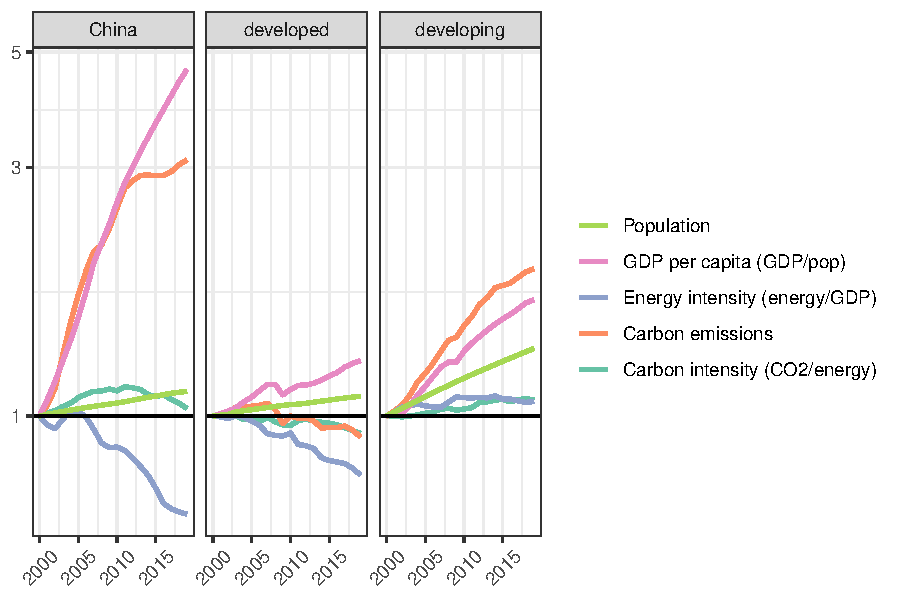
\includegraphics{Paper_files/figure-latex/unnamed-chunk-4-1.pdf}
\caption{Figure 4}
\end{figure}

Thus, in the next steps, the World Bank's Income Classification Scheme
will be used for comparison (Figure 5). In high-income countries, GDP
per capita and population are increasing only at low levels (by roughly
the factor 0.5 and 0.2 respectively). Carbon intensity and energy
intensity are decreasing, keeping carbon emissions down. The carbon
intensity is decreasing because of two factors: the fossil intensity and
the fossil share. In contrast, in low-income countries, the growth of
CO2 emissions is exceeding the growth of GDP per capita, both rising by
a factor of 2.8 and 5 respectively over the observed time span. This is
driven by a high and increasing carbon intensity. Furthermore,
population growth plays an important role in this group, and can be
considered a further driving factor of CO2 emissions. The only
contrasting factor is the decreasing energy intensity. Comparing both
groups of countries to China, one can resume that China's development
does not fit in either of the groups perfectly. Like before China's Kaya
decomposition shares similar characteristics as both groups: The small
population growth resembles the trend of high-income countries, the
dramatically decreasing energy resembles the trend of low-income
countries. Considering lower-middle income countries, they seem to show
upwards trends in any of the indicators except for energy intensity. In
comparison, in upper-middle income countries carbon emissions and GDP
per capita develop in tandem, while carbon intensity and energy
intensity only fluctuate around zero in the years from 2000 to 2019.

\begin{figure}
\centering
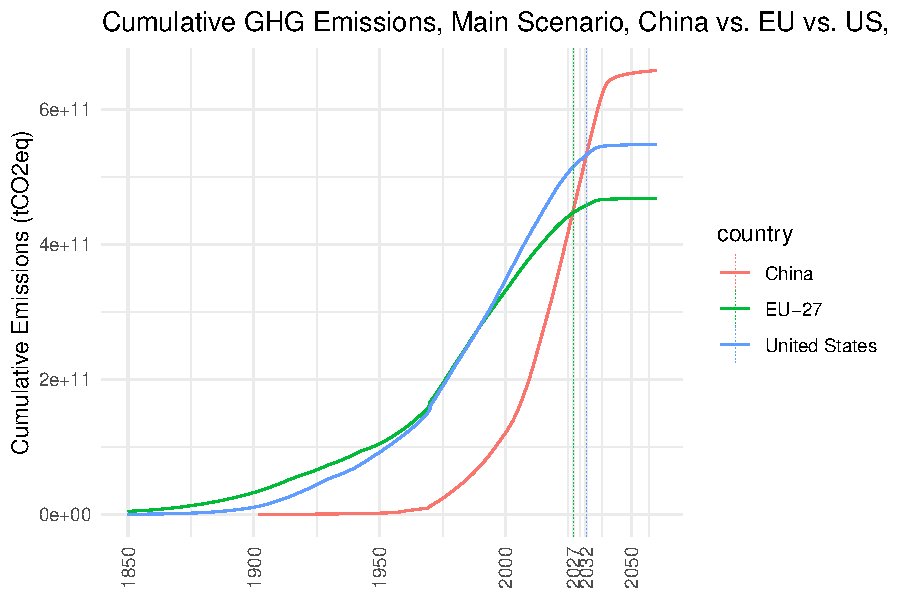
\includegraphics{Paper_files/figure-latex/unnamed-chunk-5-1.pdf}
\caption{Figure 5}
\end{figure}

To conclude, China seems to be an exception considering the driving
forces of emissions and thus cannot be assigned uniquely to any of the
studied group of countries. This is especially due to the exceptionally
high GDP growth which only recently decoupled from carbon emissions. In
terms of GDP growth rates and carbon emission growth, China can be
considered a developing nation as they base their GDP growth on growing
carbon emissions. However, the carbon and energy intensity that keep CO2
emissions down, show that China is already getting more efficient in its
production and that it has the capacity to invest in renewable energy
source. Considering only those two indicators, China can be better
compared to developed countries. Thus, it seems that China has a
responsibility to put forward this trend of efficiency gains in order to
decouple economic growth and emissions even more. To examine the status
of China in more depth, China's sectoral trends will be compared to the
two discussed classification schemes in the following. This can provide
further information on China's classification, since developing and
developed nations usually generate wealth in different economic sectors.

\hypertarget{comparison-of-chinas-sector-trends}{%
\subsubsection{Comparison of China's Sector
Trends}\label{comparison-of-chinas-sector-trends}}

In this part, sector trends of different groups of countries will be
considered using the same two categories of country groups as before. We
take into account five sectors: energy, industry, transport, AFOLU
(which in the EDGAR database only includes agricultural emissions), and
buildings. China's relative GHG emissions by sector are presented in a
stacked bar plot in Figure 6 \& 7. Most of China's emissions in 2019
came from the energy and industry sector with 44\% and 38\%
respectively. Only smaller shares are attributable to transport (6\%),
buildings (5\%) and AFOLU (6\%).

In developed countries (according to the EDGAR classification), energy
and industry still account for the majority of emissions (58\% in
total), but transport emissions play a much larger role (21\%) of the
GHG emissions than in China. This high share of transport emissions can
be accounted to the high use of private cars in developed economies. For
instance, the EU road transport accounts for 77\% of GHG emissions in
the transport sector in 2020 \citep{EEA2022}. AFOLU emissions and
emissions from buildings each account for roughly 10\% of the total GHG
emissions.\\
In contrast, in developing nations, the share of AFOLU emissions is much
larger (21\%). The high share is typically associated with the expansion
of agriculture into carbon-dense tropical forests, but also the lack of
economic development of other sectors. The share of transport, however,
is much lower than in developed countries as individual transport is not
that widely spread. The relative emissions in energy and industry are
comparable to those in developed countries as developing countries are
rapidly growing to fulfil their own and the developed countries'
consumption needs. However, absolute emissions levels are much lower.

Again, China's split of emissions does not fit in either of the two
categories. On the one hand, China's share of emissions coming from the
AFOLU sector is relatively small resembling developed country
characteristics. On the other hand, their emissions from transport
sector are small as well. This is due to the immense share of emissions
stemming from industry and energy, which reduces the share of emissions
in the other sectors.

\begin{figure}
\centering
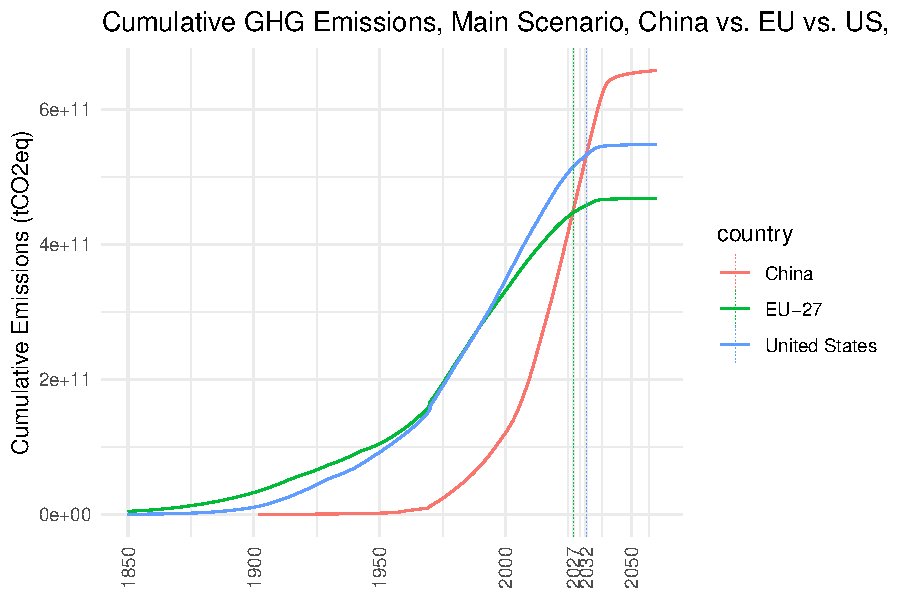
\includegraphics{Paper_files/figure-latex/unnamed-chunk-6-1.pdf}
\caption{Figure 6}
\end{figure}

As before, to get a more granular view on the split of emissions by
sector, the World Bank's classification will be consulted (Figure 7).

In this classification, differences between high-income and low-income
countries are very pronounced. While in high-income countries a major
share of emissions resulted from energy systems (37\%) in 2019, the
share of emissions from energy only accounts for 9\% of all GHG
emissions in low-income countries. This highlights an energy system
largely depending on fossil fuels in high-income countries on the one
hand, and the lack thereof in low-income countries on the other hand.
The differences are also immense considering the transport sector. In
high-income nations, 20\% of the GHG emissions stem from transport,
while in low-income countries, the share is only 7\%. However, the
biggest differences are the AFOLU emissions. High-income countries have
a share of 9\% for AFOLU emissions while in low-income countries this
sector accounts for 57\% of emissions. The reasons for these differences
were discussed above.

The emissions by sector for lower-middle and upper-middle income
countries are more similar, the only difference is that the share of
AFOLU is larger in lower-middle income countries and the share of
transport is larger for upper-middle income countries, indicating
further progress on the typical developing path of the latter country
group.

Again, China does not really fit into either of the categories due to
its very high share of emissions stemming from the energy and industry
sector. China's relative emissions from these two sectors are much
larger than in any of the other groups studied.

\begin{figure}
\centering
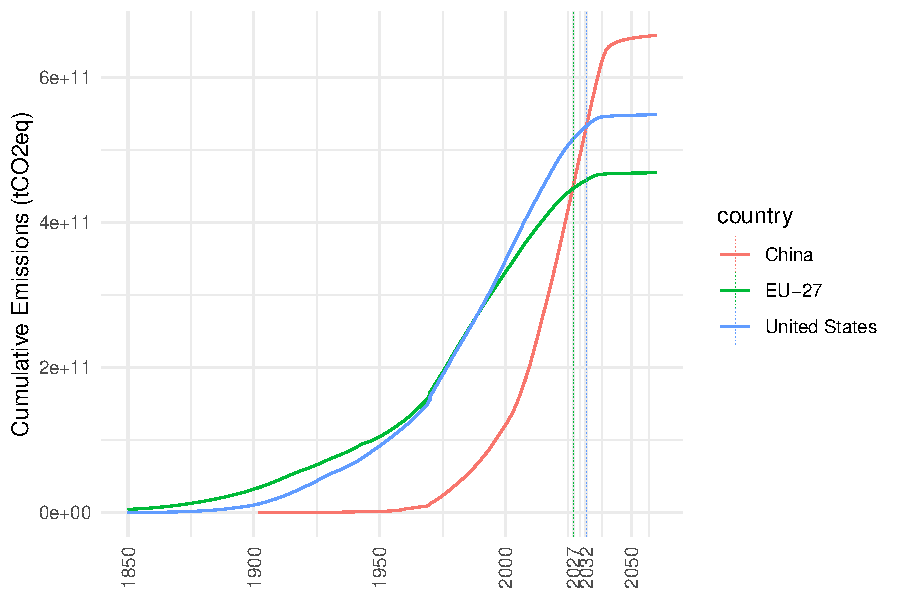
\includegraphics{Paper_files/figure-latex/unnamed-chunk-7-1.pdf}
\caption{Figure 7}
\end{figure}

As the stacked bar plot can only provide a snapshot in time and relative
emissions only tell a limited story, we will in a next step compare
China's per capita emissions by sector over time from 1970 to 2019 to
those of our four income determined country groups (Figure 8).

Comparing trends is particularly helpful, as emissions from the energy
and industry sector in China are so large, that it makes any comparison
of the remaining sectors with the potential peers very difficult.

China's AFOLU emissions per capita are relatively low and decreasing
over time, similar to the emissions in lower-middle income countries in
this sector. The AFOLU emissions per capita of high income and
upper-middle income countries are large because a relatively high
agricultural output spread over relatively small populations. In the
building sector, Chinese emissions per capita are relatively low
compared to high-income countries and rather on the same level as
upper-middle income countries. The per-capita emissions of the building
sector are high in richer countries as people require more floor space
per capita compared to lower-income countries. For transport, China's
emissions stayed on a low level until 2000 and then increased at high
speed. Now, they are comparable to per capita emissions of
upper-middle-income countries.

Considering the three sectors mentioned above, China seems to resemble
more the emissions per capita characteristics of lower-middle or
upper-middle income countries, however this is different for the energy
and industry sectors. In the energy sector, China's emissions per capita
increased up to roughly 4 tCO2eq in 2019. This is much higher than for
upper-middle income countries, in which per capita emissions stayed
relatively constant at 3 tCO2eq in 2019. In high-income countries, the
per capita emissions from energy are still higher (5 tCO2eq) in 2019
than in China, however, one can see a downward trend there. Thus, one
could argue that China can soon be compared to a high-income country
regarding its per capita energy system emissions. The same holds for the
industry sector, where this development is even more pronounced.
Emissions per capita in the industry sector in China increased massively
in the 2000s and are now at a plateau of 4 tCO2eq annually. The per
capita emissions of high-income countries in the industry sector in
contrast have decreased since the 1970s and are now at 3 tCO2eq. In the
industry China has thus already surpassed per capita emissions levels of
high-income countries and has the highest value among the five studied
panels in this sector.

\begin{figure}
\centering
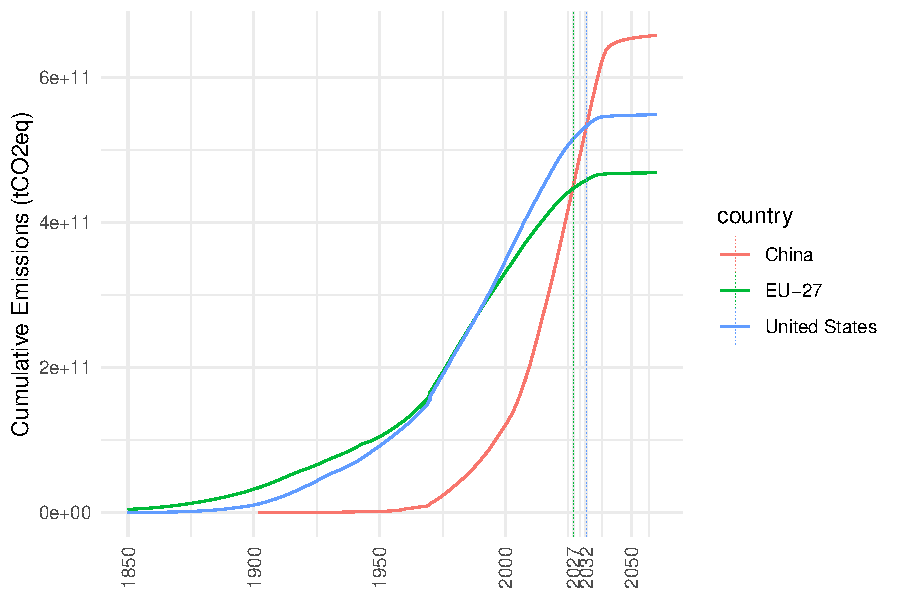
\includegraphics{Paper_files/figure-latex/unnamed-chunk-8-1.pdf}
\caption{Figure 8}
\end{figure}

\hypertarget{discussion}{%
\subsubsection{Discussion}\label{discussion}}

The prior analysis has shown that clearly classifying China as either a
developed or a developing from an emissions perspective remains
difficult.

However, what this analysis has clearly shown, is that the simple
self-characterization of China as a developing country, that is mirrored
by Sixth assessment report of the IPCC, does not do justice to the
drastic economic and emissions development China has witnessed in the
last decades. As the analysis has shown, China clearly exhibits certain
emission characteristics of developed countries in some sectors like
industry and energy systems. When it comes to agricultural per capita
emissions trends it is comparable to lower-income countries. Maybe most
importantly, in the industry sector it has the highest per capita
emissions of any of the candidates that were up for comparison.

What this analysis has undoubtedly confirmed is the realization that
China is a special case in every respect. China's unique economic
development, which has led to a five-fold increase in GDP per capita
over the past two decades, saw the country develop an energy and
industrial system that together accounts for 82\% of the country's total
emissions, a share 20\% higher than that of high-income countries.

Nevertheless, one needs to consider that development is not equally
distributed in China. The rural population has benefited significantly
less from the economic development than the urban population (East-West
divide) \citep{Knight2004}. However, the argument that one still has the
right to predominantly emissions-based development (as in 1992) is no
longer in line with China's current status as the world's biggest
emitter. Hence, China's NDC's storyline, which seeks the main
responsibility for climate change in developed nations, is too
undercomplex and does not do justice to the evolved realities.

To further investigate this issue, in the next we will predict the
future development of emissions of China and other countries and further
consider different equity metrics.

\hypertarget{chinas-equitable-share-in-climate-change-mitigation}{%
\subsection{China's Equitable Share in Climate Change
Mitigation}\label{chinas-equitable-share-in-climate-change-mitigation}}

The following chapter discusses China's equitable share in climate
change mitigation. In order to answer the research question, we will
first discuss the future development of China's emissions, to determine
when China will become the biggest cumulative emitter. For this, we
consider multiple development pathways of China in terms of emissions
and discuss China's cumulative emissions in comparison to other
countries. Moreover, we will present different rankings of absolute
emissions, per capita emissions, GDP and GDP per capita, cumulative
emissions and consumption-based CO2 emissions to discuss China's
responsibility from different perspectives.

\hypertarget{future-development-of-chinas-emissions}{%
\subsubsection{Future Development of China's
Emissions}\label{future-development-of-chinas-emissions}}

The first equity metric we consider is cumulative emissions, as China
claims historic developed countries' emissions being the main driver of
climate change. Looking at cumulative emissions from 1750 until 2019,
China is on 3 rd position, only behind the U.S. and the EU-27. According
to this, in 2019 China would already have the 3rd-largest responsibility
to reduce emissions, since it has historically emitted a total of 12.4\%
of all greenhouse gases. This is in direct contrast to the country's
claim to be less responsible for the warming climate.

Importantly, if China continues its emissions pathway, it will become
the largest cumulative emitter at some point. In order to estimate when
China will move into first place, we have modeled expected emission
trends for China as well as for the EU and the U.S. Our modelling is
based on the following assumptions:

First, for simplicity, we assume that China will reduce not only CO2
emissions, as communicated internationally, but all GHG emissions to
zero. As we have seen in section 3, Chinese emissions trends vary
strongly across sectors. Therefore, we have modelled each sector's
future emissions pathway following different assumptions. In general, we
assume a constantly declining growth rate of emissions in each sector
until a peak year starting with the 2018 to 2019 growth factor. After
the peak we consider an s-curve emissions reduction for the following
years until zero emissions are reached, as China might first use the
simple levers to reduce emissions fast and then needs to work on
emissions which are difficult to bring down.

As emissions in the AFOLU sector have already been decreasing in China,
we expect a relative flat emissions level until 2025, followed by a
decrease until zero emissions are reached in 2060. Buildings are assumed
to peak emissions in 2030 and are at zero in 2060. The energy systems
sector is expected to peak the earliest, in 2028, due to the continued
heavy roll-out of renewable energy sources in China and the experiences
from other countries decarbonization journeys. Complete decarbonization
is then assumed to be reached by 2055. We assume the industry sector to
peak by 2030 and reach complete decarbonization by 2065. As transport is
the fastest growing sector of Chinese emissions, we assume this trend to
continue (but slowed down) until 2040, and complete decarbonization in
2065.

In modeling the development of emissions for the EU-27 and the U.S., we
are guided by data from the PBL Netherlands Environmental Agency
\citep{PBL2022}. For simplicity we do not differentiate by sector but
assume a linear decrease in annual emissions up to the projected
emissions value for 2030 in both the U.S. and the EU-27. Thereafter, we
also use an s-shaped reduction curve to achieve zero emissions by 2050.

The resulting sectoral emissions pathways for each country/region are
depicted in figure xx. The resulting cumulative emissions forecasts for
the three countries/blocks are shown in figure xx. Accordingly, China
will pass the EU-27 in cumulative GHG emissions in 2027 and is projected
to pass the U.S. in 2032 . Afterwards it will be the largest cumulative
emitter.

These projections hold even when modelling each sector according to the
Chinese NDC (assuming peak years of 2030 and zero emissions by 2060). In
the NDC-scenario China will surpass the EU and US respectively in the
same years as modeled in our main scenarios, but at different emission
levels -- 452.4 GtCO2eq (main scenario) 451.8 GtCO2eq (NDC-scenario).
When projecting only CO2 emission developments1 China will surpass the
EU in 2031 and the US in 2038 according to both scenarios.

This analysis shows that maintaining targets that are ambitious in
absolute terms but relatively easy to achieve compared to China's size
and economic power, have already put China at the forefront of global
responsibility for climate change. From a cumulative emissions
perspective, China definitely has the same if not larger GHG reduction
obligations as many developed countries, especially when considering
that a majority of China's emissions were emitted after the problem of
climate change has made it on top of the global policy agenda. Moreover,
the statement of the Chinese NDC that climate change is mainly caused by
others is not tenable.

\begin{figure}
\centering
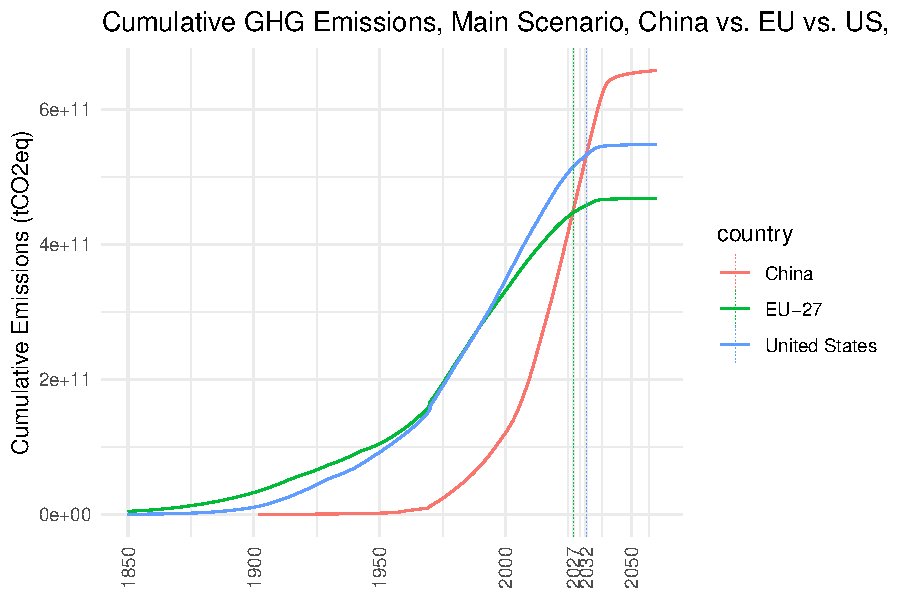
\includegraphics{Paper_files/figure-latex/unnamed-chunk-9-1.pdf}
\caption{Figure 9}
\end{figure}

However, cumulative emissions, while easily understood, are not the only
conceivable equity metric to consider when attempting to assess a
country's fair share in responding to climate change. Therefore, in the
following sub-section we investigate other equity metrics.

\hypertarget{equity-metrics}{%
\subsubsection{Equity Metrics}\label{equity-metrics}}

This chapter presents different rankings which can shed light on the
question of China's responsibility to mitigate climate change from
different angles. The following rankings always display the top 10
countries (or in case of the EU regions) in the respective category.
Furthermore, other important countries are added for comparison as well
as a category named ``Other'' which summarizes the share of all
remaining countries. The EU-27 is mentioned as a point of reference, but
emissions of the separate countries are displayed in the ranking or
summarized in the ``Other'' category. Every graph also provides
reference points for the rank position where cumulative 50 \% of global
GDP, population and emissions are surpassed.

First, we consider China's responsibility based on absolute emissions in
the year 2019 (Figure X). In the ranking, China ranks on first place
with absolute emissions of 14,219.37 Mt CO2 eq. This is more than double
of the U.S. emissions (6,266.8 Mt CO2 eq) and also close to the
emissions of all other countries that do not belong to the group of the
top 10 emitters combined (14,075.12 Mt CO2 eq). Together with the U.S.,
India and Russia, China makes up for 50\% of global emissions, but these
four countries do not produce half of the global GDP, nor do they
represent half of the world's population. This highlights that the
responsibility of these four countries to drastically reduce emissions
is high. Considering that China is producing more than double the
emissions of the U.S., China has by far the highest responsibility to
mitigate climate change from a current absolute emissions perspective.

\begin{figure}
\centering
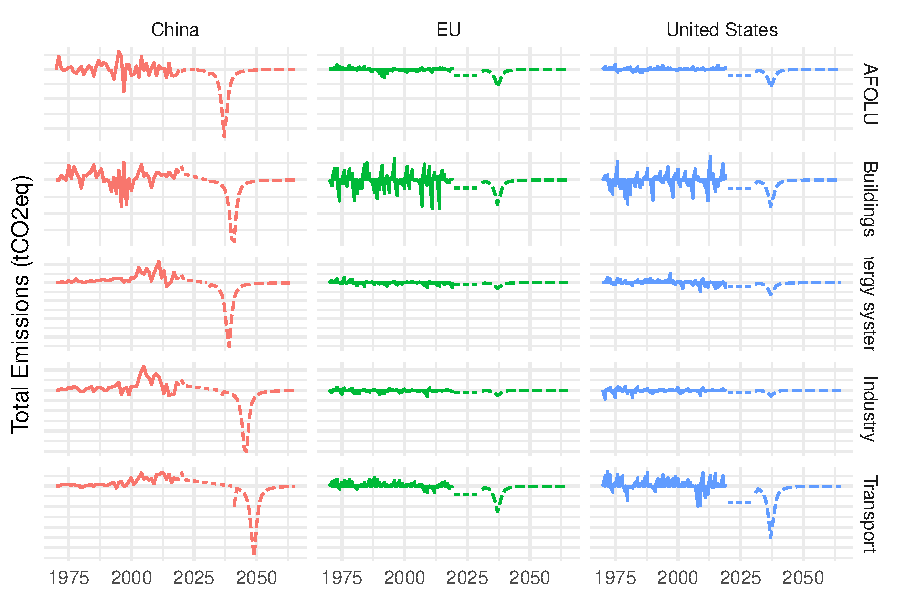
\includegraphics{Paper_files/figure-latex/unnamed-chunk-10-1.pdf}
\caption{Figure 10}
\end{figure}

Next, we consider emissions per capita (Figure x). This is important as
China is the country with the biggest population worldwide of approx.
1.4 billion people \citep{WorldBank2022c}. Looking at this ranking, it
is important to consider that the top emitters according to per capita
emissions are relatively small countries with low absolute emissions but
also small populations. Thus, when it comes to reducing absolute
emissions and fighting climate change, they can only play a minor role.
China interestingly ranks on place 43 with roughly 10t CO2 eq / capita,
before EU-27 but behind the U.S. (Ranking: 17). According to this equity
metric, China's fair share to mitigate climate change from this
perspective should be located between the share of these two
countries/groups of countries.

\begin{figure}
\centering
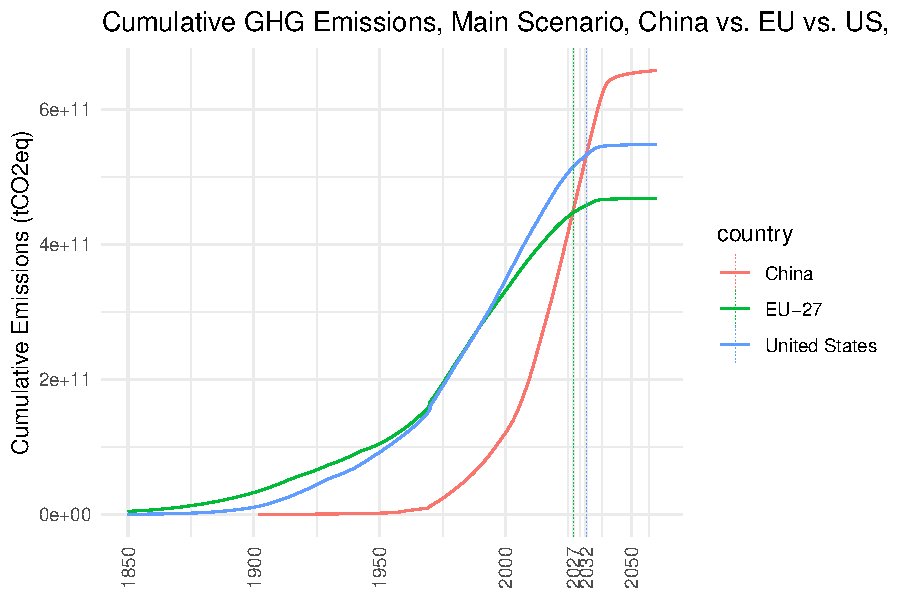
\includegraphics{Paper_files/figure-latex/unnamed-chunk-11-1.pdf}
\caption{Figure 11}
\end{figure}

Considering GDP and GDP per capita refers to the capacity of acting on
climate change, following the assumption that richer countries have more
resources available to fight climate change. As Figure XX shows, China
had the highest GDP of all countries in 2019, with USD 22.49 trillion.
Based on this, China would theoretically have to make the greatest
conribution to reduce emissions. Absolute GDP, however, is limited in
telling us about a country's actual capacity because it ignores
population size. Therefore, considering GDP per capita might be more
worthwhile. Here China only ranks 81st place in the world. Therefore,
China's responsibility is relatively low from the GDP per capita
perspective. In comparison, the U.S. rank on place 11. Countries that
are in the top 10 emitters are often relatively small countries deriving
their wealth from natural resources. Hence, they have a high
responsibility to mitigate climate change as they have the ability to
pay for climate change mitigation measures. However, their absolute
emissions are relatively small and thus an ambitious reduction might not
make a huge difference for achieving climate targets. Thus, one should
consider that these countries should specifically contribute by
providing financial aid to mitigate emissions elsewhere.

\begin{figure}
\centering
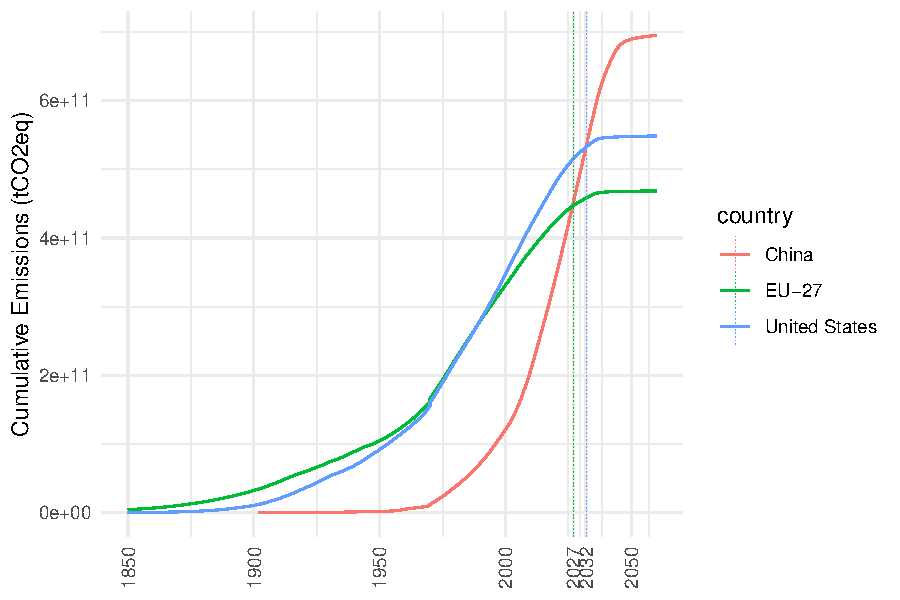
\includegraphics{Paper_files/figure-latex/unnamed-chunk-12-1.pdf}
\caption{Figure 12}
\end{figure}

\begin{figure}
\centering
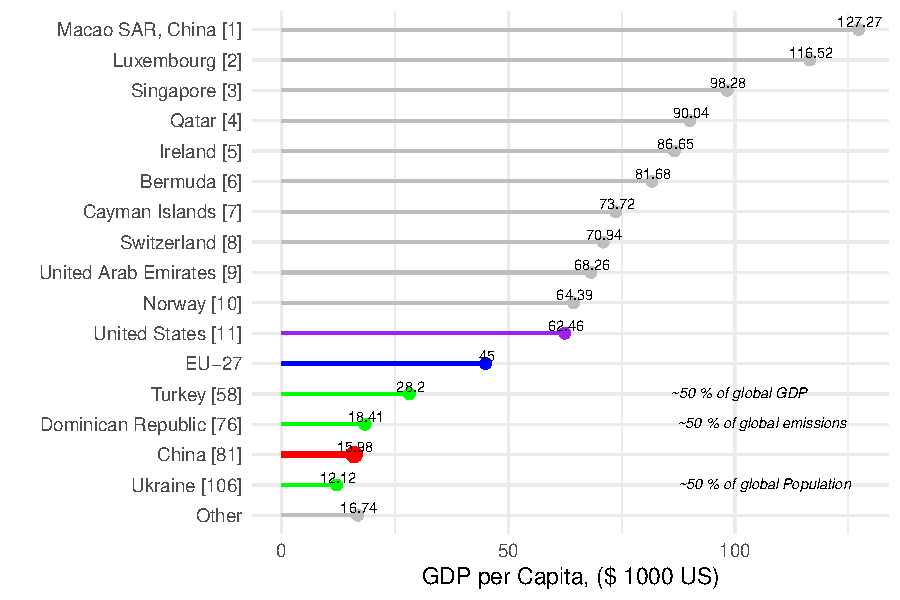
\includegraphics{Paper_files/figure-latex/unnamed-chunk-13-1.pdf}
\caption{Figure 13}
\end{figure}

\hypertarget{discussion-tbd}{%
\subsubsection{Discussion TBD}\label{discussion-tbd}}

To sum up, China has a very high responsibility to mitigate climate
change, even the highest responsibility of all countries when
considering some of the discussed equity metrics. Based on our
calculations, China is likely surpass the EU well before 2030 and the US
shortly after in 2032 in terms of cumulative emissions over all GHGs
from 1850 to 2019 and a modeling of emissions thereafter. The difference
in emissions from all GHGs to CO2 emissions highlights the importance to
extend the frame of historic respon

Therefore, China now has a major responsibility to reduce emissions
which is reinforced when considering that the country's massive
emissions growth only started after the adoption of the Kyoto Protocol
in 1997, at a time when the consequences of climate change were already
being heavily discussed.

However, we also need to consider that China only ranks on 81st. and
43rd place considering their GDP per capita and their emissions per
capita, respectively. This diminishes China's responsibility to some
extent, showing that the global community needs to grant space for
economic development to be fair. However, this economic development
should ideally be decoupled from a growth in emissions. If we look at
the per capita emissions of the countries that rank first, we see that
these are mostly very small and, from the perspective of absolute
emissions, less important countries. Although these countries might have
a high ability to pay from a per capita perspective, their overall
economic power is not high. The opposite is true for China. China ranks
first place in absolute emissions and GDP in 2019 with a great distance
to the following places.

Thus, China has one of the greatest responsibilities to reduce emissions
from a historic emissions, current emissions and economic capacity
perspective.

\hypertarget{discussion-and-conclusion-tbd}{%
\section{Discussion and Conclusion
TBD}\label{discussion-and-conclusion-tbd}}

In our analysis, we were striving to answer two research questions,
namely if China can be considered a developing country and what China's
fair share in climate change mitigation should be.

Regarding out first research question, we find that China cannot be
easily classified as a developed or developing country. This is due to
the unique economic growth (China's GDP per capita quintupled in the
last 20 years), which went hand in hand with very high energy and
industrial sectors' emissions. Comparing these to other developed
countries, one can see that China clearly exhibits these countries'
characteristics in term of sectoral emissions. However, China's
agricultural per capita emissions trends are more comparable to
lower-income countries.

Our analysis of different equity metrics for the second research
question has shown that China not only has a huge responsibility to curb
emissions, but also the financial capability to do so. The country is
the world's largest emitter in annual and cumulative terms (based on our
data) and has the highest GDP of all countries. While it is important to
acknowledge further room for development, one cannot disregard the fact
that without significant emission reductions from China, any attempt to
stay within the temperature limits of the Paris Agreement is sure to
fail.

Hence, we believe that China's fair share is much higher than what they
currently plan to do. Together with the EU-27 and the U.S., China should
bear the highest responsibility for climate change mitigation. Its
self-classification as a developing country is clearly politically
motivated, to not give in to the demands of having to do more. At the
same time, the political leadership in Beijing can present itself as a
top student in the international community by effortlessly surpassing
its own goals, as it is expected by different observers \citep{CAT2022}.

In the following, our analysis will be contrasted with two other
assessments of China's fair share -- the assessment by the Climate
Action Tracker and by the Climate Equity Monitor.

The CAT evaluates the fair share of a country based on assessments in
the literature. The results of the literature are categorized using
seven equity indicators ranging around considerations of responsibility,
capability, cost-effectiveness and equality, which are weighted equally
in the analysis. All results of the evaluated studies are then depicted
on a scale for each category and a 90\% confidence interval is built.
Based on this, the CAT develops a range of what would be a fair share
and where to categorize the different countries. The CAT values China's
share in mitigation efforts as highly insufficient. In comparison, the
U.S.'s, India's and the EU's planned policies and targets are only
considered insufficient for achieving a fair share target under the
Paris Agreement \citep{CAT2022}.

Another equity metric is developed by the Climate Equity Monitor. The
Climate Equity Monitor is the first initiative from the Global South
that tracks equity in climate action for Annex 1 and Non-Annex 1
countries. The initiative calculates the fair share of the carbon budget
by using the share of cumulative emissions based on the share in the
global population for a contemporary base year (2019). The cumulative
annual emissions of a country are calculated for the period from 1850 to
2019. Based on this, the Climate Equity Monitor calculates if a country
has a carbon debt or carbon credit. This measure is calculated as the
difference between cumulative emissions of a country and the country's
fair share of the global carbon budget already consumed. For China as a
Non-Annex 1 country, they conclude that the country has a carbon credit
of 122.4 Gt CO2eq. In comparison, India has a carbon credit of 337.6 Gt
CO2eq while the US has a carbon debt of 445 Gt CO2eq, and Russia has a
carbon debt of 125.44 Gt CO2eq \citep{CEM2022}. Accordingly, if China
kept emitting at its current rate, it would have used up its remaining
carbon credit until 2031.

It is interesting that the Climate Action Tracker and the Climate Equity
Monitor come to conclusions that can be interpreted differently. While
the latter initiative only considers cumulative emissions allowances in
relation to population size, the former's assessment benchmarks climate
targets and policies against a larger variety of equity metrics. The
remaining carbon credit derived from the Climate Equity Monitor might be
misleading to a certain degree, as it might suggest little urgency to
act, especially when comparing the credit numbers to the debt numbers of
other countries. The CAT's assessment, while being methodically more
sophisticated, better communicates the implications of current emission
reduction targets and respective policies from an equity perspective.

Our analysis has the following limitations: We only consider cumulative
emissions from 1850-2019, but the consideration of other time periods
could also be conceivable. The problem of climate change caused by
anthropogenic greenhouse gas emissions has only been known since the
1970s, and since the 1990s there has been a dedicated international
process to address the problem. Against this background, an additional
consideration of cumulative emissions in these time periods might be
worthwhile. For a comprehensive assessment of China's fair share, it
would have also been interesting to discuss further equity metrics such
as a ranking of consumption-based emissions. However, this was not
possible for us, as our data only included consumption-based data for
approx. 100 countries and crucially missing the US, making a comparison
less meaningful.

\appendix
\section*{Appendix}
\addcontentsline{toc}{section}{Appendix}
\renewcommand{\thesubsection}{\Alph{subsection}}
\newcommand{\subsectionbreak}{\clearpage\phantomsection}
\numberwithin{table}{subsection}

\normalsize

\hypertarget{session-info-rstudio}{%
\subsection{Session Info (RStudio)}\label{session-info-rstudio}}

\footnotesize

\begin{itemize}\raggedright
  \item R version 4.2.1 (2022-06-23 ucrt), \verb|x86_64-w64-mingw32|
  \item Running under: \verb|Windows 10 x64 (build 22621)|
  \item Matrix products: default
  \item Base packages: base, datasets, graphics, grDevices, methods,
    stats, utils
  \item Other packages: dplyr~1.0.10, eurostat~3.7.10, forcats~0.5.2,
    ggplot2~3.3.6, ggridges~0.5.4, imputeTS~3.3, kableExtra~1.3.4,
    magrittr~2.0.3, openxlsx~4.2.5, pacman~0.5.1, plotly~4.10.1,
    purrr~0.3.4, readr~2.1.2, readxl~1.4.1, stringr~1.4.1,
    tibble~3.1.8, tidyr~1.2.1, tidyverse~1.3.2, WDI~2.7.8
  \item Loaded via a namespace (and not attached): assertthat~0.2.1,
    backports~1.4.1, bibtex~0.5.0, broom~1.0.1, cellranger~1.1.0,
    class~7.3-20, classInt~0.4-8, cli~3.4.0, colorspace~2.0-3,
    compiler~4.2.1, countrycode~1.4.0, crayon~1.5.1, curl~4.3.2,
    data.table~1.14.2, DBI~1.1.3, dbplyr~2.2.1, digest~0.6.29,
    e1071~1.7-11, ellipsis~0.3.2, evaluate~0.16, fansi~1.0.3,
    farver~2.1.1, fastmap~1.1.0, forecast~8.18, fracdiff~1.5-2,
    fs~1.5.2, gargle~1.2.1, generics~0.1.3, ggtext~0.1.2, glue~1.6.2,
    googledrive~2.0.0, googlesheets4~1.0.1, grid~4.2.1, gridtext~0.1.5,
    gtable~0.3.1, haven~2.5.1, here~1.0.1, highr~0.9, hms~1.1.2,
    htmltools~0.5.3, htmlwidgets~1.5.4, httr~1.4.4, jsonlite~1.8.0,
    KernSmooth~2.23-20, knitr~1.40, labeling~0.4.2, lattice~0.20-45,
    lazyeval~0.2.2, lifecycle~1.0.2, lmtest~0.9-40, lubridate~1.8.0,
    modelr~0.1.9, munsell~0.5.0, nlme~3.1-157, nnet~7.3-17,
    parallel~4.2.1, pillar~1.8.1, pkgconfig~2.0.3, plyr~1.8.7,
    proxy~0.4-27, quadprog~1.5-8, quantmod~0.4.20, R6~2.5.1,
    Rcpp~1.0.9, RefManageR~1.4.0, regions~0.1.8, reprex~2.0.2,
    rlang~1.0.5, rmarkdown~2.16, rprojroot~2.0.3, rstudioapi~0.14,
    rvest~1.0.3, scales~1.2.1, stinepack~1.4, stringi~1.7.8,
    svglite~2.1.0, systemfonts~1.0.4, tidyselect~1.1.2,
    timeDate~4021.104, tools~4.2.1, tseries~0.10-52, TTR~0.24.3,
    tzdb~0.3.0, urca~1.3-3, utf8~1.2.2, vctrs~0.4.1, viridisLite~0.4.1,
    webshot~0.5.3, withr~2.5.0, xfun~0.33, xml2~1.3.3, xts~0.12.2,
    yaml~2.3.5, zip~2.2.1, zoo~1.8-11
\end{itemize}

\normalsize
\singlespacing
\listoffigures
\listoftables

\def\bibpreamble{All online resources were last accessed on 12 December 2022.}
\footnotesize

  \bibliography{packages.bib}

\end{document}
